\documentclass[11pt,a4paper]{article}

\usepackage[margin=1in]{geometry}
\usepackage[utf8]{inputenc}
\usepackage{amsmath,amssymb}
\usepackage{graphicx}
\usepackage{booktabs}
\usepackage{longtable}
\usepackage{caption}
\usepackage{subcaption}
\usepackage{tabularx}
\usepackage{array}
\usepackage{makecell}
\usepackage{siunitx}
\usepackage[hidelinks]{hyperref}
\usepackage[capitalise]{cleveref}

\sisetup{
  group-separator = {\,},
  input-ignore = {,},
  detect-all,
}

\title{Adverse Events in Psychedelic-Assisted Therapies: A Meta-Analysis}
\author{}
\date{\today}

\begin{document}
\maketitle

\begin{abstract}
% Abstract to be completed separately.
\end{abstract}

\section{Methods}
\subsection{Study design and registration}
This meta-analysis followed a predefined analytic protocol to evaluate adverse events (AEs) reported in controlled trials of psychedelic compounds. No prospective registration (e.g., PROSPERO) was filed; the protocol, data exports, and analytic scripts are archived within the project repository to enable reproducibility.

\subsection{Eligibility criteria and information sources}
Eligible studies were randomized or otherwise controlled human trials evaluating 3,4-methylenedioxymethamphetamine (MDMA), lysergic acid diethylamide (LSD), psilocybin, or ayahuasca that reported systematically collected AEs. Inactive placebo arms served as the preferred reference; if unavailable, the lowest active dose per molecule-specific hierarchy was selected. Records were excluded when dosing information was unclear, AE capture was unsystematic, or designs were uncontrolled, case-series, or animal based. Searches encompassed major databases (e.g., PubMed), trial registries (e.g., ClinicalTrials.gov), and grey literature resources (e.g., Cochrane Central) without date or language restrictions, supplemented by backward citation chasing of eligible reports.

\subsection{Data extraction and items}
Structured templates captured study identifier, molecule, arm identifier, number of participants per arm, harmonised AE term (\texttt{ae\_term}), assessment window (acute \emph{session} vs. longer-term \emph{follow-up}), participant counts experiencing each AE (observed or back-calculated from proportions), and administered dose in milligrams (with conversions from mg/kg where necessary). Extraction was performed independently by two analysts with discrepancies resolved by consensus. Arm-level contributions to the pooled evidence base, including contrasts and unique dose levels, are summarised in \Cref{tab:study-characteristics}.

\subsection{Risk of bias assessment}
Risk of bias was planned using Cochrane domains covering randomization, allocation concealment, blinding, and attrition. Several historical reports lacked sufficient detail for complete scoring; consequently, narrative descriptions were retained for contextual interpretation, and no quantitative down-weighting by risk-of-bias category was applied.

\subsection{Synthesis methods}
Active arms were paired against their designated reference arms to form $2\times2$ tables per contrast. Primary effect measures were risk ratios; risk differences were substituted in models that required stabilization, following \texttt{metafor} defaults. Random-effects models using restricted maximum likelihood (REML) generated pooled estimates overall and per \texttt{ae\_term}. Between-study heterogeneity was summarised using $\tau^2$ (REML) and $I^2$. Leave-one-out diagnostics were produced when at least three contrasts were available. Small-study bias assessments (funnel plots and Egger tests) were planned for pooled estimates with $k\geq10$.

\subsection{Dose--response and subgroup modelling}
Dose--response relationships were evaluated via meta-regression of study contrasts, fitting prespecified linear terms and restricted cubic splines when dose coverage spanned at least three non-reference levels per molecule. Time-window stratification (session vs. follow-up) was incorporated either through stratified models or interaction terms. Per-AE spline overlays were generated when multiple molecules reported the same harmonised AE term to permit cross-molecule comparisons.

\subsection{Sensitivity analyses}
Sensitivity analyses comprised leave-one-out recalculations, separate pooling by assessment window, and molecule-specific contrasts. Additional exploratory summaries contrasted session and follow-up slopes alongside per-AE significance patterns, linking to the comparative tables in \Cref{tab:cmp_topline,tab:cmp_ae_molecule} and the session-versus-follow-up visualisation in \Cref{fig:session-followup}.

\subsection{Statistical software}
All analyses were executed in R (version 4.3 or later). Key packages included \texttt{metafor} for random-effects estimation, \texttt{dplyr} and \texttt{tidyr} for data manipulation, \texttt{splines} and \texttt{dosresmeta} for dose--response modelling, and \texttt{ggplot2} with \texttt{patchwork} for figure assembly. Full scripts and exported artefacts are bundled with the repository to support replication.

\IfFileExists{tables/study_characteristics.tex}{%
  \begin{table}[ht]
    \centering
    \caption{Arm-level contrasts contributing to session and follow-up analyses by molecule. Dashes indicate windows without available contrasts.}
    \label{tab:study-characteristics}
    \begin{tabular}{lcccc}
\toprule
Molecule & $k_{\text{session}}$ & $k_{\text{follow-up}}$ & Doses (session) & Doses (follow-up) \\
\midrule
Ayahuasca & 16 & \textemdash & 1 & \textemdash \\
LSD & 149 & 108 & 6 & 5 \\
MDMA & 160 & 58 & 6 & 2 \\
Psilocybin & 162 & \textemdash & 3 & \textemdash \\
\bottomrule
\end{tabular}

  \end{table}
}{}

\section{Results}
\subsection{Study selection}
Screening identified controlled trials of MDMA, LSD, psilocybin, and ayahuasca reporting harmonised AE outcomes. Common exclusion reasons included uncontrolled designs, absent AE capture, and non-human evidence. The final dataset retained both session and, when available, follow-up assessments aligned to the reference-arm policy described above.

\subsection{Study characteristics}
Included trials spanned a wide dosing range and observation windows. Session-level contrasts were available for all four molecules, while follow-up contrasts were predominantly reported for LSD and MDMA. \Cref{tab:study-characteristics} summarises the number of contrasts and distinct dose levels informing each synthesis stratum.

\subsection{Primary pooled synthesis}
Random-effects pooling across molecules indicated elevated AE risk relative to reference arms, as depicted in the forest plot in \Cref{fig:overall-forest}. Molecule- and window-specific significance patterns, including the number of AE terms reaching statistical significance, are documented in \Cref{tab:cmp_topline}. Session analyses for LSD, MDMA, and psilocybin achieved statistical significance, whereas follow-up estimates were more uncertain because of sparse contrasts.

\IfFileExists{figures/forest_combined_all_molecules.pdf}{%
  \begin{figure}[ht]
    \centering
    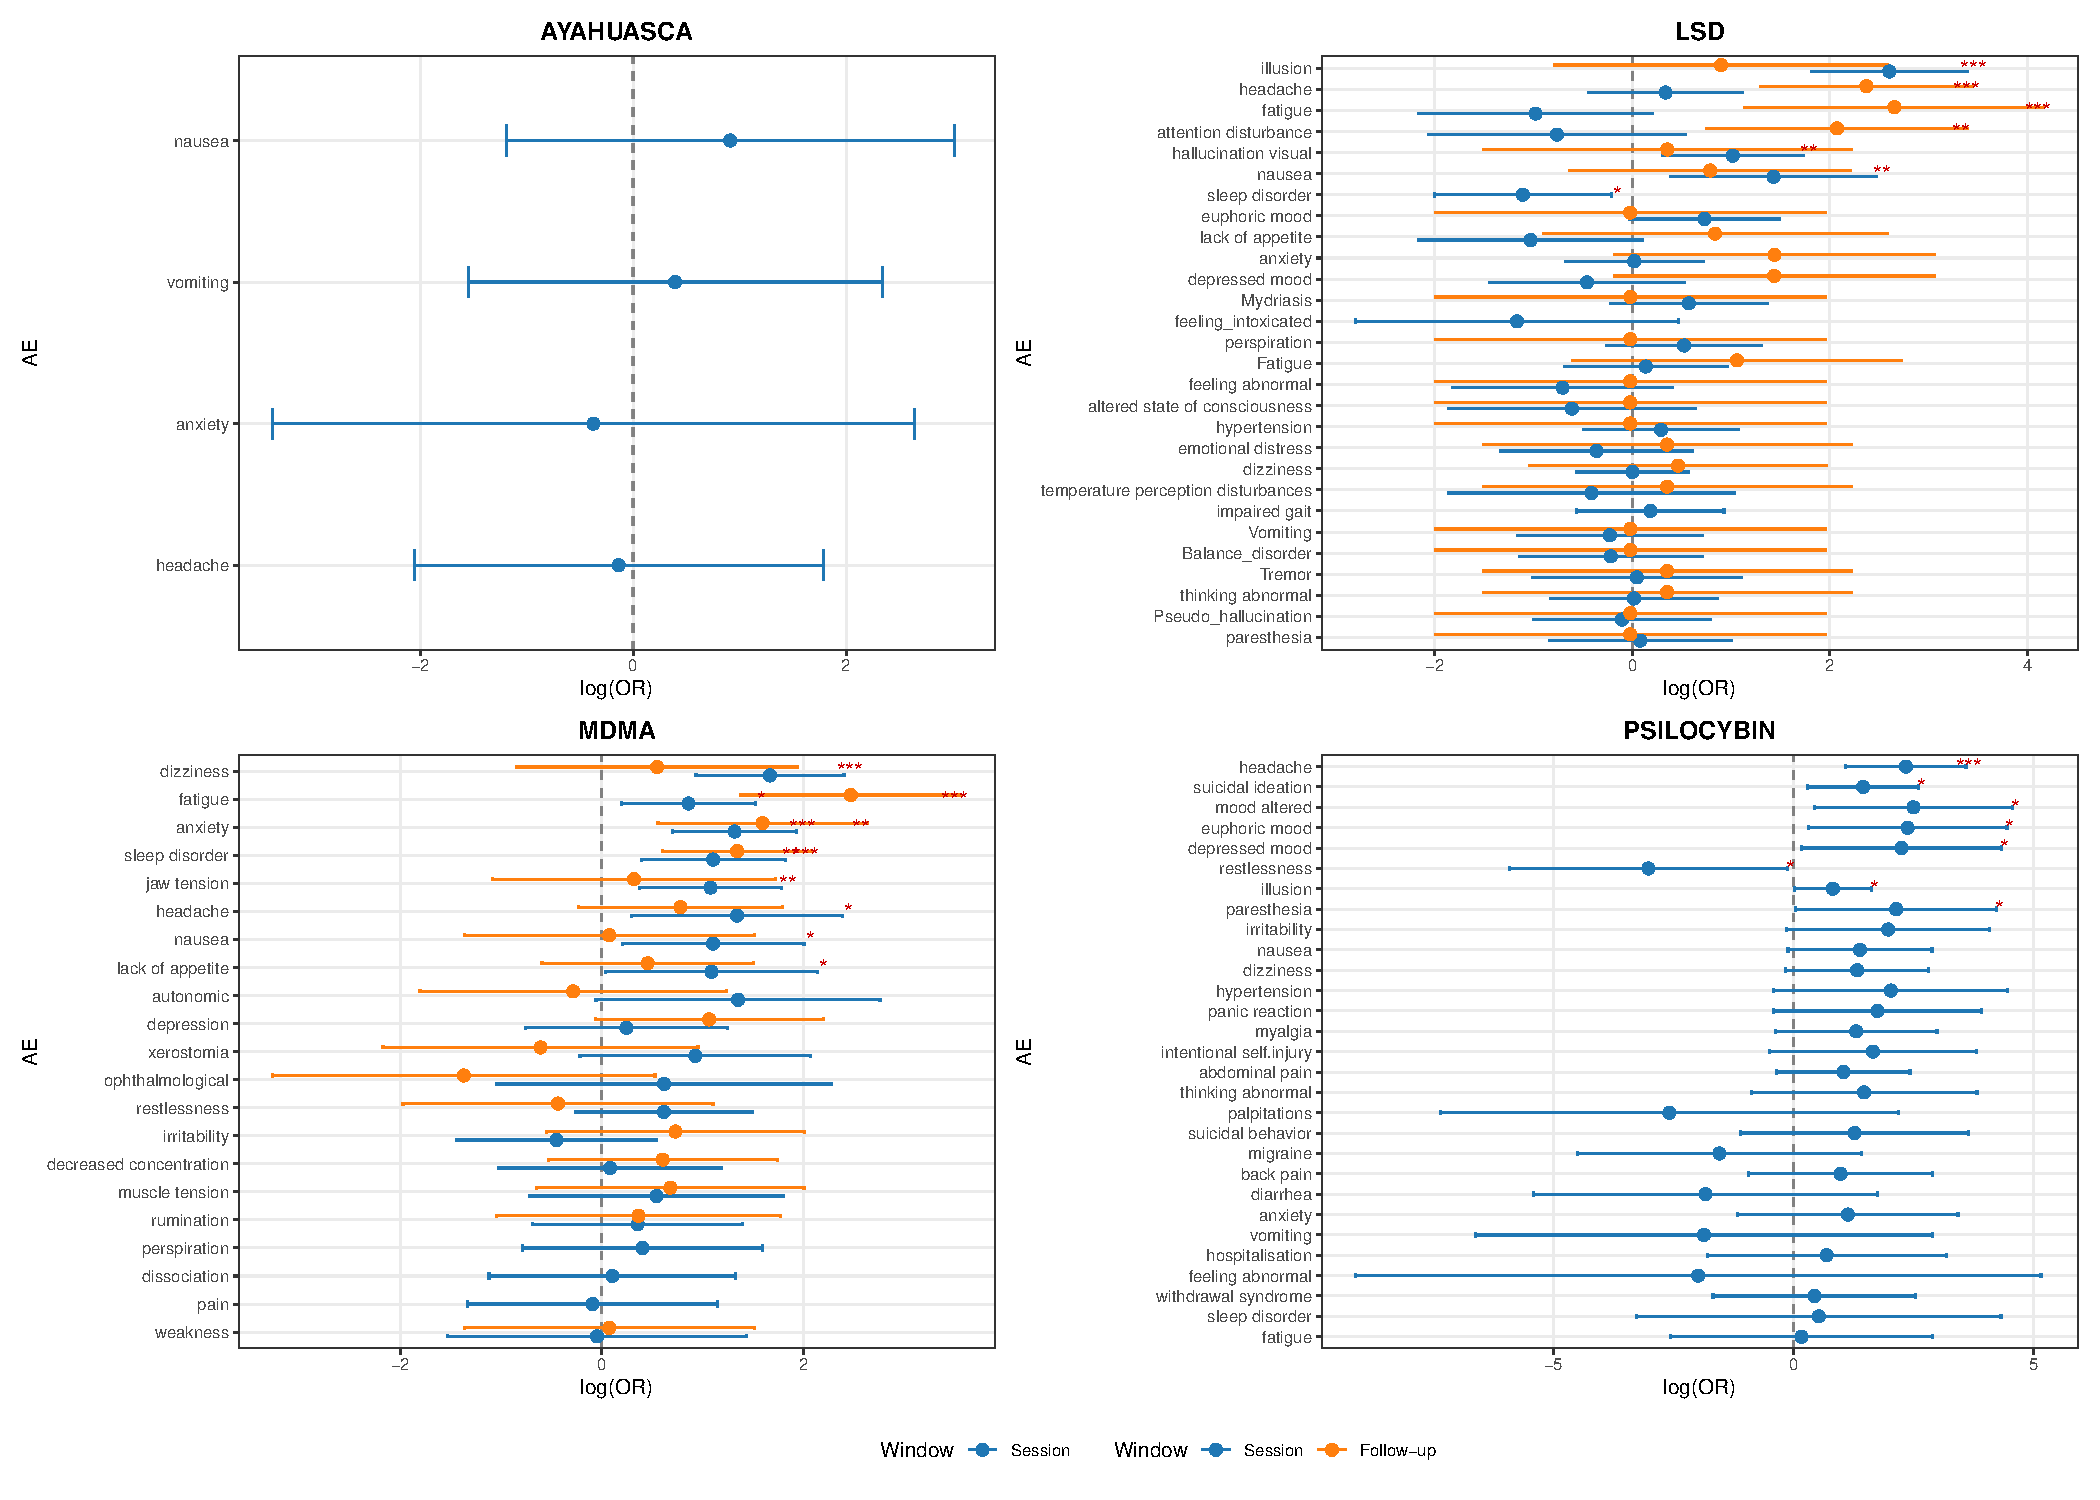
\includegraphics[width=\linewidth]{figures/forest_combined_all_molecules.pdf}
    \caption{Random-effects pooled AE risk ratios across molecules and assessment windows.}
    \label{fig:overall-forest}
  \end{figure}
}{}

\IfFileExists{../results_compare/tables/compare_topline_publication.tex}{%
  \begin{table}[ht]
\centering
\caption{Overall significance by molecule (session vs follow-up) and number of significant AE.}
\label{tab:cmp_topline}
\begin{tabular}{lllll}
\toprule
Molecule & Overall (session) & Overall (follow-up) & # significant AE (session) & # significant AE (follow-up) \\
\midrule
LSD & p=0.00084 *** & p=0.00235 ** & 2 &  0 \\
MDMA & p=1.47e-13 *** & p=0.0565  & 2 &  0 \\
Psilocybin & p=3.94e-11 *** &  & 1 &  \\
\bottomrule
\end{tabular}
\end{table}


}{}

\subsection{Per-adverse-event findings}
Harmonised per-AE models highlighted a subset of AE terms with statistically significant elevations. For LSD, nausea and headache reached significance, whereas MDMA analyses identified headache and depressive symptoms. Psilocybin models emphasised fatigue as the most consistent signal. The corresponding $p$-values are reported in \Cref{tab:cmp_ae_molecule}. Session-level dose--response overlays in \Cref{fig:per-ae-overlays} illustrate cross-molecule trajectories for shared AE terms.

\IfFileExists{figures/master_dr_by_ae-session.pdf}{%
  \begin{figure}[ht]
    \centering
    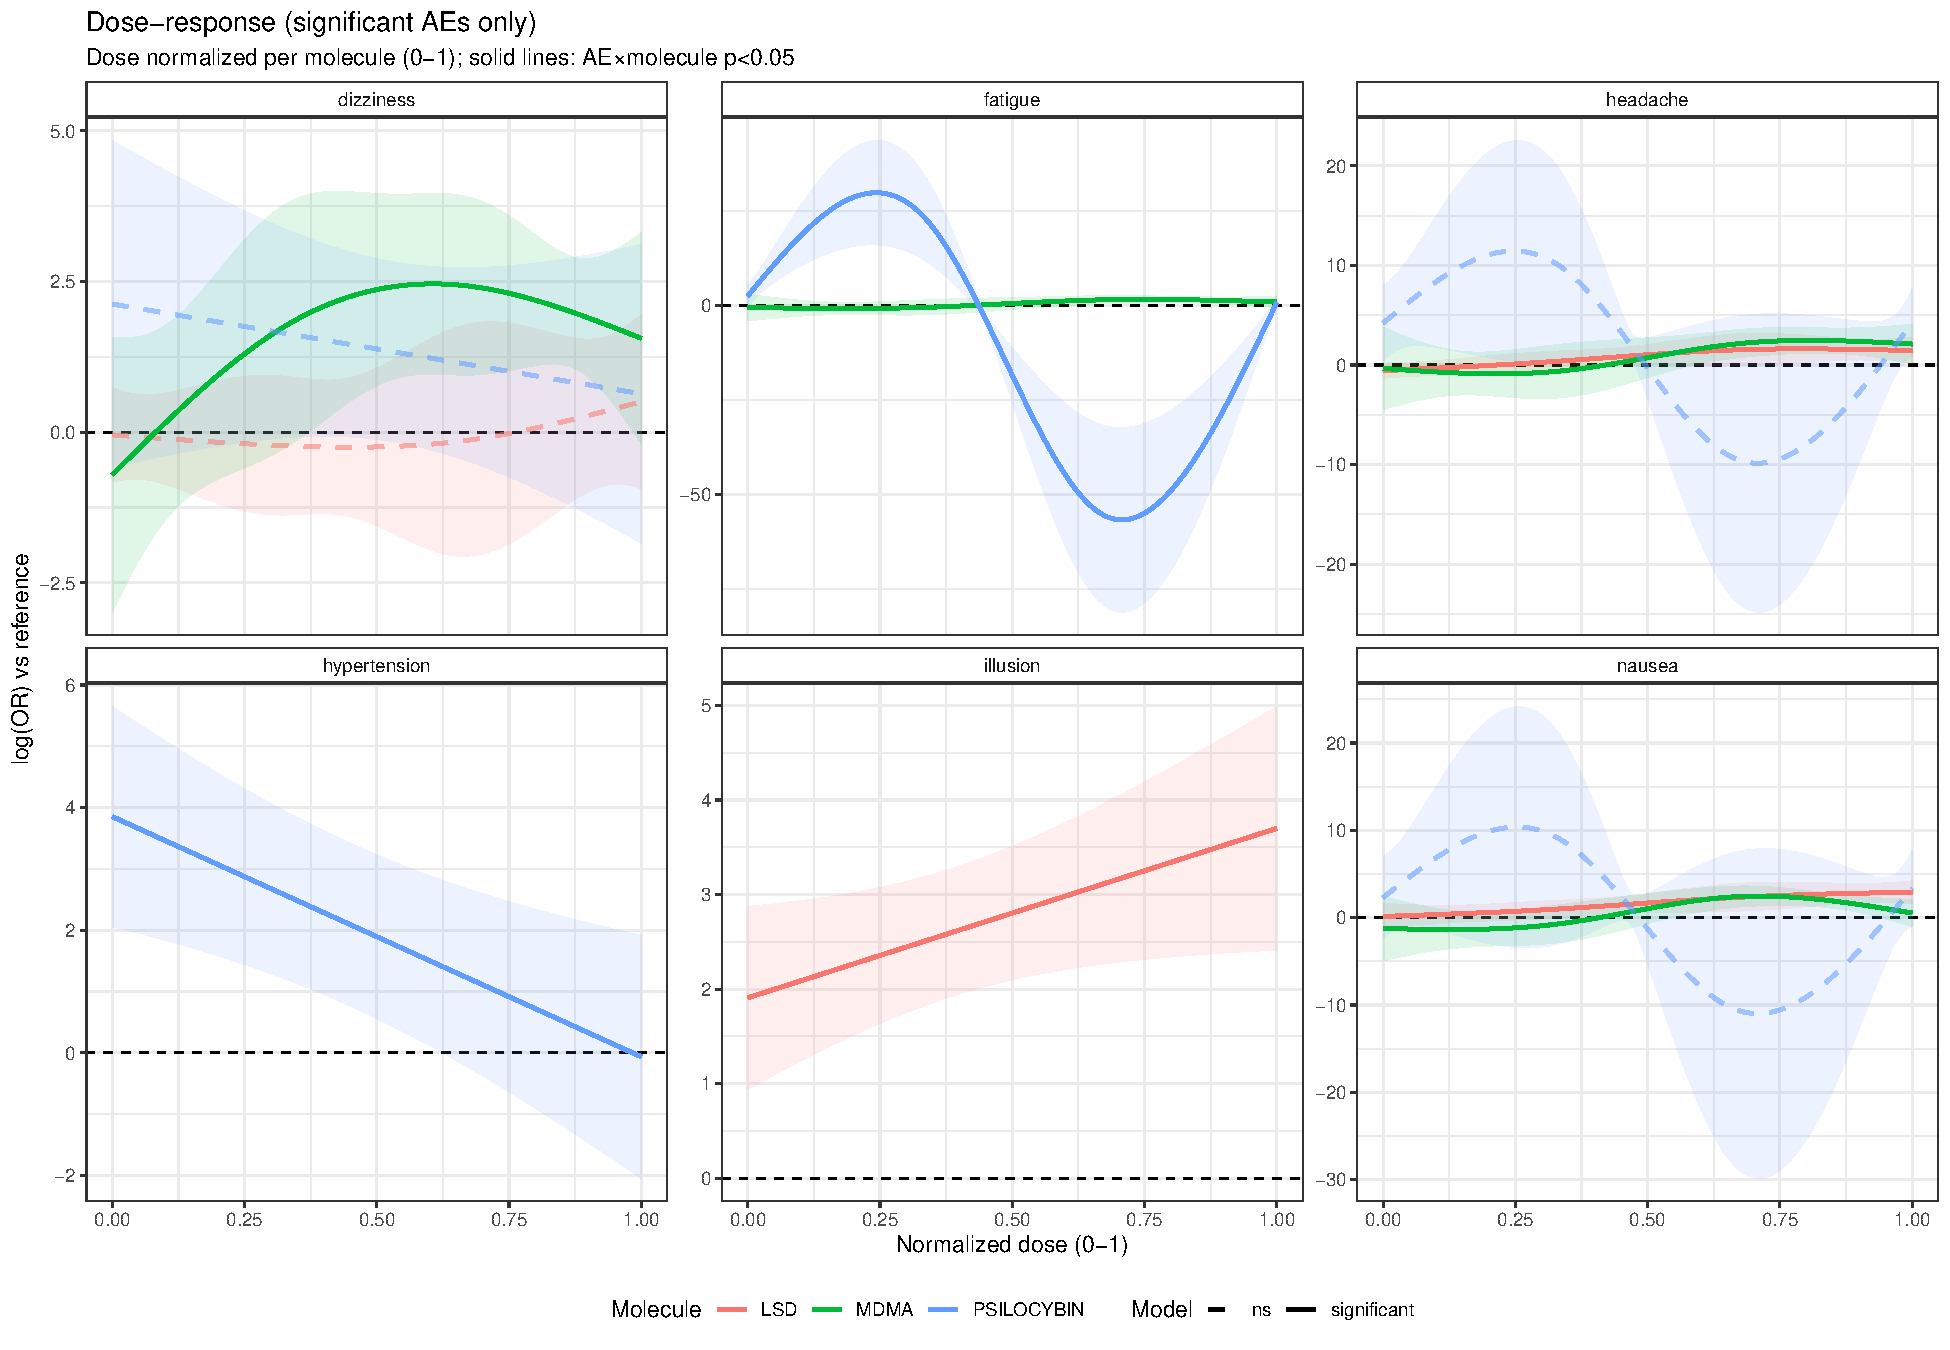
\includegraphics[width=\linewidth]{figures/master_dr_by_ae-session.pdf}
    \caption{Session-level dose--response overlays for harmonised AE terms observed across multiple molecules.}
    \label{fig:per-ae-overlays}
  \end{figure}
}{}

\IfFileExists{../results_compare/tables/compare_by_ae_molecule.tex}{%
  \begin{table}[ht]
\centering
\caption{Per-AE comparison by molecule: session vs follow-up p-values.}
\label{tab:cmp_ae_molecule}
\begin{tabular}{llll}
\toprule
molecule & ae_term & session & follow \\
\midrule
LSD & anxiety & p=0.713  &  \\
LSD & attention disturbance & p=0.526  & p=0.15  \\
LSD & dizziness & p=0.89  & p=0.912  \\
LSD & emotional distress & p=0.256  &  \\
LSD & feeling abnormal & p=0.372  &  \\
LSD & headache & p=0.0104 * & p=0.629  \\
LSD & nausea & p=0.025 * & p=0.885  \\
LSD & perspiration & p=0.511  &  \\
LSD & temperature perception disturbances & p=0.774  &  \\
LSD & thinking abnormal & p=0.662  &  \\
MDMA & anxiety & p=0.0724  &  \\
MDMA & autonomic & p=0.0719  &  \\
MDMA & depression & p=0.0456 * &  \\
MDMA & dissociation & p=0.362  &  \\
MDMA & dizziness & p=0.147  &  \\
MDMA & fatigue & p=0.159  &  \\
MDMA & headache & p=0.00654 ** &  \\
MDMA & irritability & p=0.284  &  \\
MDMA & jaw tension & p=0.491  &  \\
MDMA & lack of appetite & p=0.156  &  \\
MDMA & muscle tension & p=0.509  &  \\
MDMA & nausea & p=0.336  &  \\
MDMA & ophthalmological & p=0.196  &  \\
MDMA & pain & p=0.129  &  \\
MDMA & perspiration & p=0.072  &  \\
MDMA & restlessness & p=0.374  &  \\
MDMA & rumination & p=0.709  &  \\
MDMA & sleep disorder & p=0.0643  & p=0.539  \\
MDMA & xerostomia & p=0.836  &  \\
Psilocybin & abdominal pain & p=0.502  &  \\
Psilocybin & anxiety & p=0.591  &  \\
Psilocybin & fatigue & p=2.54e-06 *** &  \\
Psilocybin & headache & p=0.207  &  \\
Psilocybin & nausea & p=0.537  &  \\
Psilocybin & suicidal ideation & p=0.462  &  \\
\bottomrule
\end{tabular}
\end{table}


}{}

\subsection{Dose--response relationships}
Dose--response meta-regression revealed molecule-specific patterns (\Cref{fig:dose-response}). MDMA demonstrated approximately monotonic increases in AE risk with higher doses, whereas LSD and psilocybin displayed non-linear trajectories consistent with restricted cubic spline fits. Ayahuasca contributed multiple contrasts but only one unique session dose and was therefore not modelled for continuous dose effects.

\IfFileExists{figures/master_dr_by_molecule-session.pdf}{%
  \begin{figure}[ht]
    \centering
    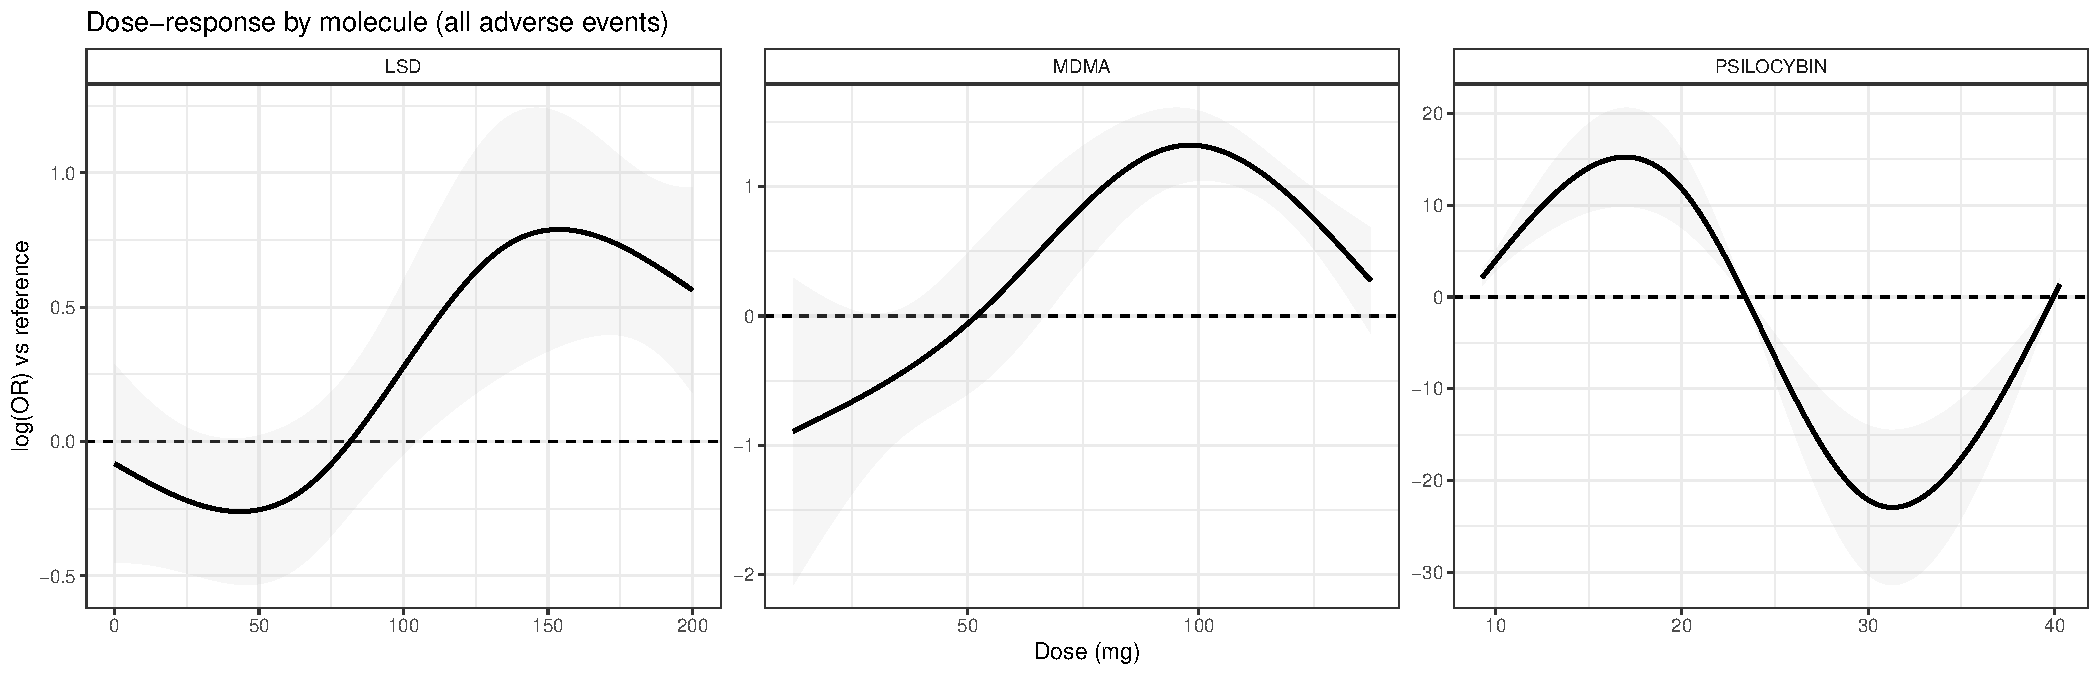
\includegraphics[width=\linewidth]{figures/master_dr_by_molecule-session.pdf}
    \caption{Session-level dose--response curves from spline meta-regressions for each molecule.}
    \label{fig:dose-response}
  \end{figure}
}{}

\subsection{Session versus follow-up comparisons}
Comparisons between session and follow-up windows suggested attenuation of AE signals at later assessments, as visualised in \Cref{fig:session-followup}. The tabulated contrasts in \Cref{tab:cmp_topline,tab:cmp_ae_molecule} show that several AE terms with session-level significance did not retain statistical support at follow-up, reflecting both diminished sample sizes and fewer reported contrasts.

\IfFileExists{figures/dr_session_vs_followup.pdf}{%
  \begin{figure}[ht]
    \centering
    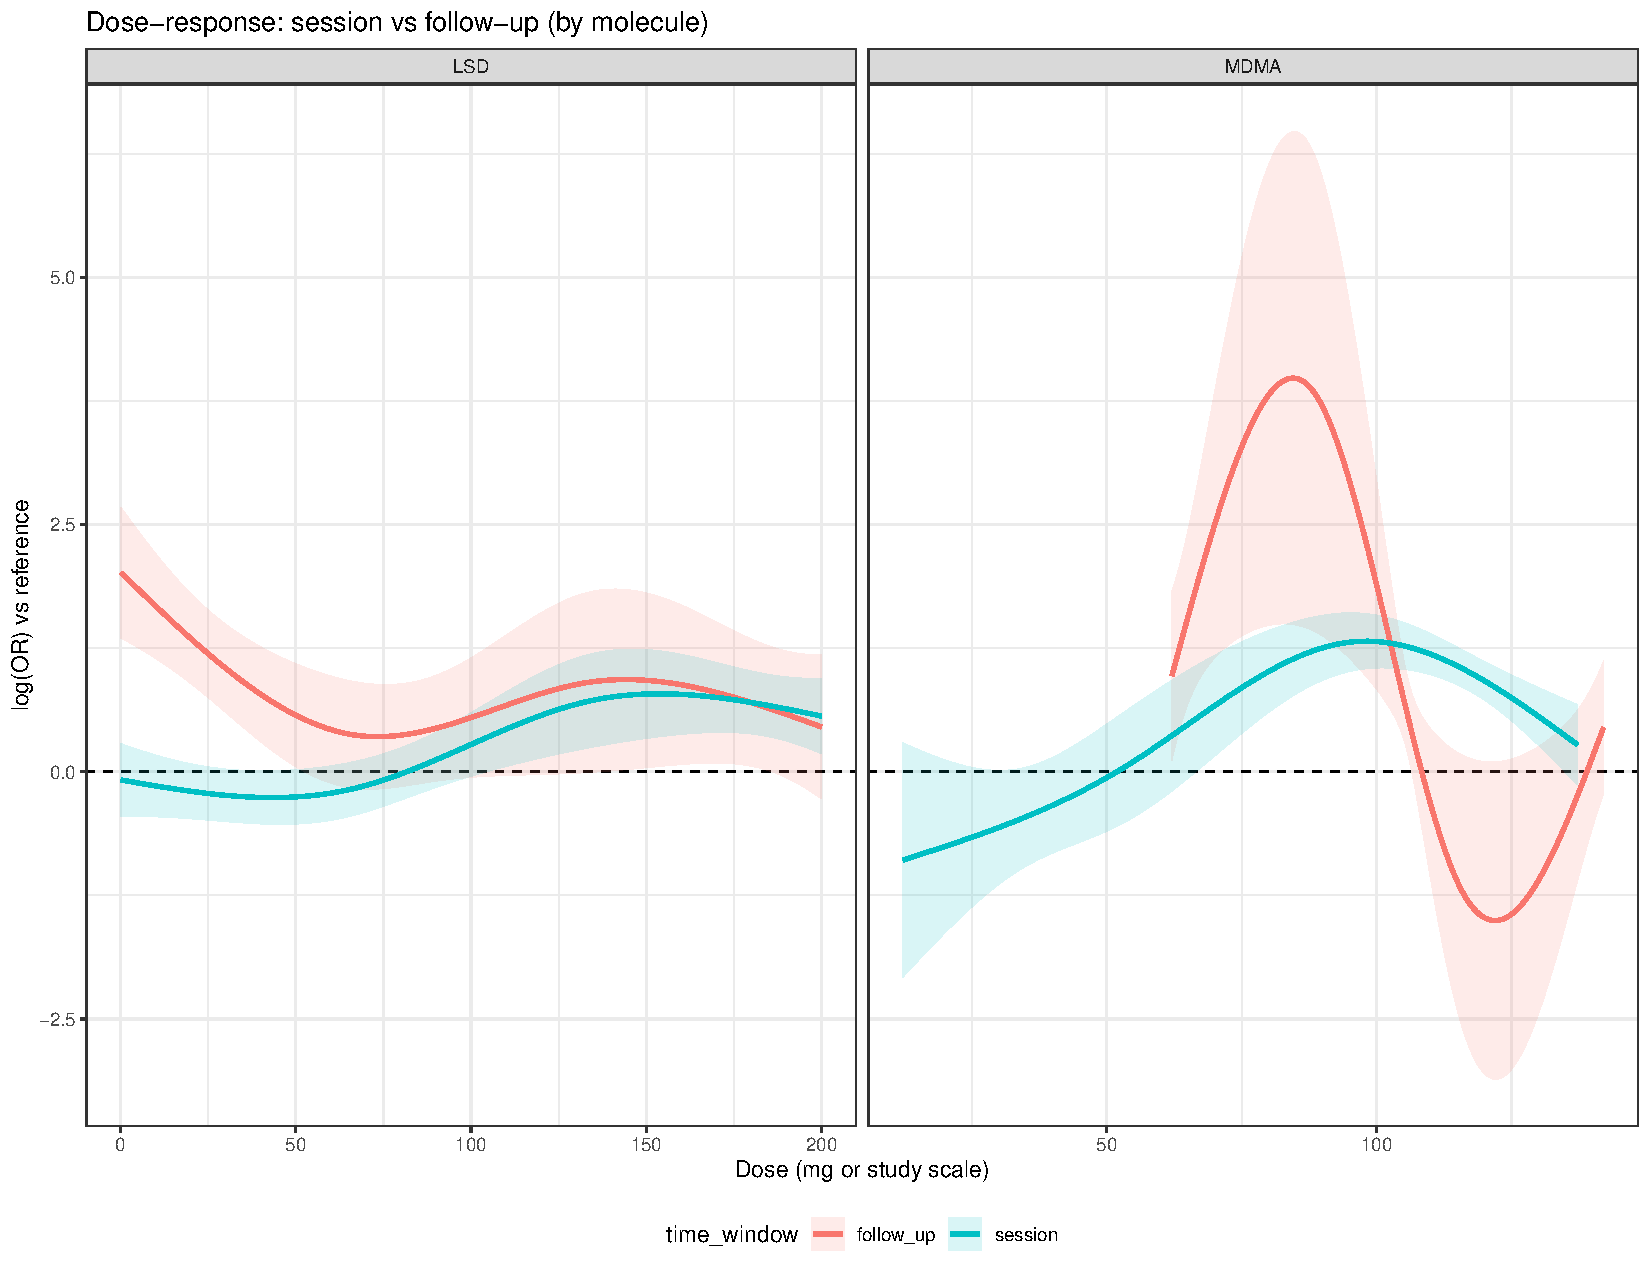
\includegraphics[width=\linewidth]{figures/dr_session_vs_followup.pdf}
    \caption{Comparison of session and follow-up dose--response slopes across molecules.}
    \label{fig:session-followup}
  \end{figure}
}{}

\section{Discussion}
% To be developed.

\end{document}
